\documentclass[a4paper,10pt,reqno,oneside]{amsart}
\usepackage[small]{caption}
%\usepackage[usenames,dvipsnames]{color}
%\usepackage[colorlinks=TRUE,linkcolor=Black,urlcolor=Black,citecolor=Black,pagebackref=TRUE,]{hyperref} %Have to change href email.
\usepackage{amsfonts,fancyhdr,graphicx,lastpage,rotating,multirow,fixltx2e, stfloats,txfonts,palatino,url,xcolor,multicol,hanging, setspace,lscape, paralist, changepage,subcaption,array,verbatim,setspace, siunitx, tikz, flafter}
\usepackage[pagewise,displaymath, mathlines]{lineno}
\usepackage{epstopdf}

\renewcommand{\theequation}{eqn \arabic{equation}}
\makeatletter
\def\tagform@#1{\maketag@@@{\ignorespaces#1\unskip\@@italiccorr}}
\makeatother




%\usepackage[nolists, nomarkers]{endfloat}
\linenumbers
\doublespacing

\usepackage[sort&compress,comma]{natbib}



% This declares the unit "animals". Also redefined days to be whole word *(not sure if thats what is needed.

\DeclareSIUnit{\animals}{animals}
\DeclareSIUnit{\day}{days}





\usepackage{etoolbox}

\def\r{4}
\def\o{0.3}
\def\lwr{-1.3*\r}
\def\upr{1.3*\r}
\def\gap{0.2}
\def\arrowSz{0.5}
\def\angRad{0.6}
\definecolor{arrowCol}{rgb}{0.5,0.5,0.5}
\definecolor{sensCol}{rgb}{0,0,1}
\definecolor{callCol}{rgb}{1,0,0}

\tikzstyle{profile}=[ultra thick, red]



\newlength{\x}
\newlength{\y}

\newcommand{\call}[1]{ % callAngle
        \fill[opacity=\o, red] (-{\r*sin(#1/2)}, \lwr) rectangle ({\r*sin(#1/2)}, \upr);       
}

\newcommand{\profileOne}[2]{ % sensor width, x1

	\setlength{\x}{#2 pt}
	\setlength{\y}{#1 pt}
	\ifboolexpr{%
		test {\ifdimless{0.5\y}{\x}} 
		and
		test{\ifdimless{\x}{360 pt -0.5\y}} 
	}{
		\pgfmathsetmacro{\leftProf}{max({\r*cos(#2 - #1/2)},{\r*cos(#2 + #1/2)})};
	}{
		\pgfmathsetmacro{\leftProf}{\r};
	}
	\draw[profile]  (0,0)  -- (180:\leftProf)
                        (0,0)  -- (0:\r);  
}



\newcommand{\sensorOne}[2]{ % sensorAngle, x1
	\setlength{\x}{#2 pt}
	\setlength{\y}{#1 pt}
	\ifboolexpr{%
		test {\ifdimless{0.5\y}{\x}} 
		and
		test{\ifdimless{\x}{360 pt -0.5\y}} 
	}{
		\pgfmathsetmacro{\leftProf}{max({\r*cos(#2 - #1/2)},{\r*cos(#2 + #1/2)})};
	}{
		\pgfmathsetmacro{\leftProf}{\r};
	}
        \fill[opacity=\o, blue] (-\leftProf, \lwr) rectangle ({\r}, \upr);       
}

\newcommand{\segmentOne}[2]{ % sensor width, x1
	\draw[] (0,0) -- ++(180 + #1/2 - #2:\r)
     	        (0,0) -- ++(180 - #1/2 - #2:\r);
	\draw[] (0,0) ++(180 + #1/2 - #2:\r) arc (180 + #1/2 - #2:180 - #1/2 - #2:\r);
}

\newcommand{\directionArrowOne}[3]{ % callAngle, sensorAngle, x1
	\setlength{\x}{#3 pt}
	\setlength{\y}{#2 pt}
	\ifboolexpr{%
		test {\ifdimless{0.5\y}{\x}} 
		and
		test{\ifdimless{\x}{360 pt - 0.5\y}} 
	}{
		\pgfmathsetmacro{\leftPoi}{max({\r*cos(#3 - #2/2)},{\r*cos(#3 + #2/2)})};
	}{
		\pgfmathsetmacro{\leftPoi}{\r};
	}
        \pgfmathsetmacro{\rightPoi}{max({\r*sin(#1/2)},{\r)})}
        \fill[ arrowCol ] (-\leftPoi, \lwr-\gap) -- (\rightPoi, \lwr-\gap) -- ({(-\leftPoi+\rightPoi)/2},\lwr-\gap - \arrowSz) -- cycle;

}


\newcommand{\profileTwo}[2]{ % sensor width, x2
        \pgfmathsetmacro{\pLen}{{2*\r*sin(#1/2)*sin(#2)}}
        \draw[profile] (0,0)  ++ (#2 - #1/2:\r) -- ++(180:\pLen) ;
	\draw[profile] (0,0) ++(#2 + #1/2:\r) ++ (0,-\angRad) arc (-90:-(90 - #2):\angRad);
        \node[above right] at (#2 + #1/2:\r) {$x_2$}
}

\newcommand{\sensorTwo}[2]{ % sensorAngle, x2
        \fill[opacity=\o, blue] ({\r*cos(#1/2 + #2)}, \lwr) rectangle ({\r*cos(#2 - #1/2)}, \upr);       
}

\newcommand{\segmentTwo}[2]{ % sensor width, x2
	\draw[] (0,0) -- ++(#2 - #1/2:\r)
     	        (0,0) -- ++(#2 + #1/2:\r);
	\draw[] (0,0) ++(#2 - #1/2:\r) arc (#2 - #1/2:#2 + #1/2:\r);
	\draw[] (0,0) ++(#2 - #1/2:\r) -- (#2 + #1/2:\r);
}

\newcommand{\directionArrowTwo}[3]{ % callAngle, sensorAngle, x2
        \pgfmathsetmacro{\leftPoi}{min({-\r*sin(#1/2)},{\r*cos(#2/2 + #3)})}
        \pgfmathsetmacro{\rightPoi}{max({\r*sin(#1/2)},{\r*cos(#3 - #2/2)})}
        \fill[ arrowCol ] (\leftPoi, \lwr-\gap) -- (\rightPoi, \lwr-\gap) -- ({(\leftPoi+\rightPoi)/2},\lwr-\gap - \arrowSz) -- cycle;

}

\newcommand{\profileThree}[2]{ % sensorAngle, x3
        \pgfmathsetmacro{\pLen}{{\r*sin(#2)}}
        \draw[profile] (0,0) ++ (90 - #2:\r) -- ++(180:\pLen) ;
	\draw[profile] (0,0) ++  (0,\angRad) arc (90:90 - #2:\angRad);
        \node[below right] at (0,0) {$x_3$}
}

\newcommand{\sensorThree}[2]{ % sensorAngle, x3
        \fill[opacity=\o, blue] (0, \lwr) rectangle ({\r*sin(#2)}, \upr);       
}

\newcommand{\segmentThree}[2]{ % sensorAngle, x3
	\draw[] (0,0) -- ++(90 - #2 + #1:\r)
     	        (0,0) -- ++(90 - #2:\r);
	\draw[] (0,0) ++(90 - #2 + #1:\r) arc (90 - #2 + #1:90 - #2:\r);
	\draw[] (0,0) ++(90 - #2 + #1:\r) -- (90 - #2:\r);
}


\newcommand{\directionArrowThree}[3]{ % callAngle, sensorAngle, x3
        \pgfmathsetmacro{\leftPoi}{min({-\r*sin(#1/2)},{0})}
        \pgfmathsetmacro{\rightPoi}{max({\r*sin(#1/2)},{\r*sin(#2)})}
        \fill[ arrowCol ] (\leftPoi, \lwr-\gap) -- (\rightPoi, \lwr-\gap) -- ({(\leftPoi+\rightPoi)/2},\lwr-\gap - \arrowSz) -- cycle;

}



\newcommand{\profileFour}[2]{ % sensor width, x4
        \draw[profile] (0,0)  -- ++(0:\r) ;
	\draw[profile] (0,0) ++ (\angRad,0) arc (0:-#2:\angRad);
        \node[above right] at (0,0) {$x_4$}
}

\newcommand{\sensorFour}[2]{ % sensorAngle, x4
        \fill[opacity=\o, blue] (0, \lwr) rectangle ({\r}, \upr);       
}

\newcommand{\segmentFour}[2]{ % sensor width, x4
	\draw[] (0,0) -- ++(#1 - #2:\r)
     	        (0,0) -- ++(-#2:\r);
	\draw[] (0,0) ++(#1 - #2:\r) arc (#1 - #2:-#2:\r);
	\draw[] (0,0) ++(#1 - #2:\r) -- (-#2:\r);
}

\newcommand{\directionArrowFour}[3]{ % callAngle, sensorAngle, x4
        \pgfmathsetmacro{\leftPoi}{min({-\r*sin(#1/2)},0)}
        \pgfmathsetmacro{\rightPoi}{max({\r*sin(#1/2)},{\r)})}
        \fill[ arrowCol ] (\leftPoi, \lwr-\gap) -- (\rightPoi, \lwr-\gap) -- ({(\leftPoi+\rightPoi)/2},\lwr-\gap - \arrowSz) -- cycle;

}





\newcommand{\fullOne}[3]{ % call, sensor, x4
        \call{#1};
        \sensorOne{#2}{#3};
        \directionArrowOne{#1}{#2}{#3};
        \segmentOne{#2}{#3};
        \profileOne{#2}{#3};
}



\newcommand{\fullTwo}[3]{ % call, sensor, x2
        \call{#1};
        \sensorTwo{#2}{#3};
        \directionArrowTwo{#1}{#2}{#3};
        \segmentTwo{#2}{#3};
        \profileTwo{#2}{#3};
}

\newcommand{\fullThree}[3]{ % call, sensor, x3
        \call{#1};
        \sensorThree{#2}{#3};
        \directionArrowThree{#1}{#2}{#3};
        \segmentThree{#2}{#3};
        \profileThree{#2}{#3};
}



\newcommand{\fullFour}[3]{ % call, sensor, x4
        \call{#1};
        \sensorFour{#2}{#3};
        \directionArrowFour{#1}{#2}{#3};
        \segmentFour{#2}{#3};
        \profileFour{#2}{#3};
}




\begin{document}


\title[Estimating abundance using camera traps and acoustic detectors]{Ideal gas models for estimating abundance using camera trap and acoustic sensor count data}
\maketitle

\subsection*{ Running title: Estimating abundance using camera traps and acoustic detectors}

\subsection*{ Word count:}

\subsection*{ Authors:\\}
Tim C.D. Lucas\textsuperscript{1,2,3*}, Elizabeth Moorcroft\textsuperscript{1,4,5}, %Kate E. Jones\textsuperscript{2,5}, Marcus J. Rowcliffe\textsuperscript{5}, Robin Freeman\textsuperscript{5}\\


\subsection*{ Addresses:\\}
1 CoMPLEX, University College London, Physics Building, Gower Street, London, WC1E 6BT, UK\\ 
2 Centre for Biodiversity and Environment Research within Genetics, Evolution and Environment, UCL, Gower Street, London, WC1E 6BT, UK\\ 
3 Department of Statistical Science, University College London, Gower Street, London, WC1E 6BT, UK\\ 
4 Department of Computer Science, University College London, Gower Street, London, WC1E 6BT, UK\\ 
5 Institute of Zoology, Zoological Society of London, Regents Park, London, NW1 4RY, UK


\subsection*{ Corresponding authors:\\}
Tim C.D. Lucas,\\
CoMPLEX,\\
University College London,\\
Gower Street,\\
London,\\
WC1E 6BT, \\
UK\\
timcdlucas@gmail.com\\


Elizabeth Moorcroft,\\
CoMPLEX,\\
University College London,\\
Gower Street,\\
London,\\
WC1E 6BT, \\
UK\\
e.moorcroft@ucl.ac.uk\\

Kate E. Jones,\\
CBER,\\
University College London,\\
Gower Street,\\
London,\\
WC1E 6BT, \\
UK\\
kate.e.jones@ucl.ac.uk\\

\clearpage


%max word count 250 words. 

\section{Abstract}
\subsection*{Point 1:}   It is currently difficult to estimate population densities using data collected using camera traps and acoustic detectors. Current methods often require individual identification or an estimate of the distance between animal and sensor. An approach without these requirements, `ideal gas' models, have so far only been extended for camera traps with a small range of detection angles and acoustically detected animals with directional calls currently do not fit the assumptions of gas models.

\subsection*{Point 2:} We have generalised the `ideal gas' model so that animal density can be estimated from count data obtained using acoustic detection of animals with directional calls or data from camera trap surveys. We simulated a sensor survey of an animal population moving through space. From these surveys we estimated animal density using our new models and compared this to the known input density of animals to test the validity of the new models.

\subsection*{Point 3:} The new models can be used to estimate animal density from surveys with any combination of detection angles and call directionality. We find that the models give an unbiased estimate of density. The precision of the estimate increases with survey effort. We find that for a high density population, 24 hours of surveying will give a good estimate of density. %The estimate remains unbiased under a range of assumptions about animal movement. 

\subsection*{Point 4:} We conclude that these models provide an effective method to estimate animal density from sensor count data. We anticipate that surveys of acoustically direction species, or camera trap surveys, which before could only give relative metrics of population size will now be able to estimate population density.   As sensors such as camera traps and acoustic detectors become cheaper and more practical these models will be increasingly useful for monitoring animal populations across broad spatial, temporal or taxonomic scales.

\subsection{Keywords}
Acoustic detection, animal density, random encounter model, bat detector.

\section{Introduction}

An estimate of the size of an animal population is one of the fundamental measures needed in ecology and conservation. The absolute size of a population has important implications for a range of issues such as genetic diversity \citep{o1985genetic, fischer2000genetic, willi2005threefold} and sensitivity to stochastic fluctuations \citep{wright1983stochastic, richter1972extinction}. Random sampling can be easily used as a relative measure to track population changes. However, using a population sample to estimate absolute density can be difficult as detectability, in terms of probability of being in close proximity to an animal and in terms of detecting it once it is nearby, can skew estimates \citep{jennelle2002use, foster2012critique}.

The methods for sampling populations are varied. Traditionally, human surveyors collecting data were the primary method but technological sensors, such as camera traps \citep{ahumada2011community, rowcliffe2008surveys} and acoustic detectors \citep{ofarrel1999comparison, jones2011indicator, mellinger2007fixed} are becoming increasingly used to survey animal populations.  Technological sensors are growing in popularity, as they are efficient, relativity cheap and non-invasive \citep{gese2001monitoring, o2003crouching, silveira2003camera}. With respect to efficiency, the use of autonomous sensors allows for surveys over continental areas, for years or decades. 

Some species are much more easily detected or identified by acoustic detectors. For example, while bat identification by hand requires much training, methods are being developed to automatically identify species from their calls \citep{walters_2012, Adams_2010}. With respect to distance (or the radius of detection), large Cetaceans are loud enough to detected from tens of \SI{}{\kilo \meter} away, further than is possible visually \cite{clark1995application, barlow2005estimates, mcdonald2004difar}.  


The problem of converting sampled count data to estimates of density remains. The preferred method for estimating density is capture-recapture methods \citep{leslie1953estimation,schwarz1999} if individuals can be recognised e.g. \citep{karanth1995, trolle2003estimation, soisalo2006estimating, trolle2007camera}. If individual recognition is impossible but the distance between animal and sensor can be estimated transect methods can be used to estimate density, although these often ignore animal movement which may bias estimates \citep{barlow2005estimates, marques2011estimating}. Finally, methods for density estimation, based on ideal gas models (originally formulated by physicists to estimate contact rates between molecules) have been developed \citep{yapp1956theory, Hutchinson_Waser_2007}. The gas model has been modified for use with camera traps with an angle of detection (the maximum angle from centre that an animal can still be detected)  of $\pi/2$ radians \citep{rowcliffe2008estimating}. These models have not been formulated to account for the reduced detection that occurs when an animals' call is directional.

In this study we create a general model, as an extension to the camera trap model of \cite{rowcliffe2008estimating}, to estimate absolute abundance from count data from acoustic detectors or camera traps  where the sensor angle can vary from 0 to $2\pi$ radians, and the acoustic signal given off from the animal can be directional (we call the width of an animals acoustic call the call angle). Specifically, we break the model into many different models for different values of the sensor angle and the call angle. We then derive the gas model as an illustration of the general principle and then derive one of the more complicated models. The remaining derivations are included in the supplementary material (S1). We tested the model using simulations in order to assess the validity of the models and in order to give suggestions for best practice. Specifically, we test that the analytical model can accurately predict density when the assumptions of a homogeneous environment and straight-line animal movement are met and that the accuracy of the model is not affected by changes in the assumptions we make about animal movement. We also quantify the effect of sampling effort, radius of detection, call angle and directionality, animal movement speed and density on the precision of the analytical models.




\begin{comment}
\begin{itemize}
\item Monitoring the size of populations is necessary for maintaining biodiversity.
\item Monitoring can be done in different ways, by a direct count or through taking samples. \citep{pollock2002large}
\item Methods for collecting samples can vary from human surveys to sensor records, such as the results from cameras or sound recorders placed throughout an environment. 
\item Sensors are growing in popularity, as they are efficient, relativity cheap and non-invasive. \citep{gese2001monitoring}
\item These species are often difficult to capture on camera, but are easier to detect using an acoustic sensor \citep{rogers2013density}, such as bats \citep{ofarrel1999comparison}, whales \citep{mcdonald1999passive}, and potentially for species such as monkeys. 
\item Samples collected from sensors can then be used in methods like REM or Capture-Recapture in order to estimate density of the population.
\item Current methods are not suitable for all species, so some species have no, or unreliable, population information. Because the width of the sensor can be greater than 90, and because the animal may give off a directional signal 
\item We are going to extend REM methods so that it can be used with acoustic data as well as data collected via camera traps
\end{itemize}



\subsection{Aims}

\begin{itemize}
\item  In this study we created a general model, as an extension to the REM, to estimate absolute abundance from count data from acoustic or visual sensors. Where the angle of detection of the sensor can vary from 0 to \SI{360}{\degree}, and the signal given off from the animal can be between 0 and \SI{360}{\degree}.
\item  We tested the model using simulations in order to:
\begin{itemize}
\item Access the validity, i.e. that the bias is equal to 0
\item  To be able to give suggestions for best practice
\end{itemize}
\end{itemize}

\subsection{Hypotheses}

\begin{itemize}
\item The analytical model can accurately predict density when the assumptions of a homogeneous environment and straight-line animal movement are met.
\item The accuracy of the model is not affected by changes in the movement model, however the precision of the analytical models are affected
\item The precisions of the analytical models are also affected by sampling effort, radius of detection, call angle and detection angle, animal speed and density.
\end{itemize}
\end{comment}

\section{Methods}

\subsection{Analytical Model}

Our derivations follow the model presented by \cite{rowcliffe2008estimating} which extends the gas model to model camera trap surveys. This model is derived assuming a sensor with a detection angle less than $\pi/2$ radians and so the sensor is modelled as a circular segment with a central angle between 0 and  $\pi/2$ named  $\theta$ (see Table~\ref{t:paras} for a list of symbols.) We call this segment the sensor region. Furthermore, as \cite{rowcliffe2008estimating}  modelled a camera trap, an animal can be detected from any angle as long as it is within the segment shaped sensor region; an in front of the camera trap but moving away from it can be detected. We however want to relax this assumption to allow for acoustically detected animals with directional calls. We therefore model the animal as having an associated call angle $\alpha$. In general we are aiming to derive models for any sensor angle, $ \theta$, between 0 and $2\pi$ and any call angle, $ \alpha$, between 0 and $2\pi$. Although these two parameters vary continuously, there are many models which need to be derived and analysed separately. The values of $\theta$ and $\alpha$ for these different models are shown in Figure~\ref{f:regions}. In this section we show the derivation for the gas model (which is the simplest of the models) and outline the general process for deriving other models by working through one example. 



\begin{table}[t]
\centering
\begin{tabular}{lll}
Symbol 	& Description & Units\\\hline
$v$		& Velocity & \SI{}{\meter\per\second}\\
$\theta$	& Angle of detection & Radians \\
$\alpha$	& Animal call/beam width & Radians \\
$r$ 		& Detection distance & Metres\\
$p$ 		& Average profile width & Metres\\
$t$		& Time & Seconds\\
$z$		& Number of detections & \\
$D$		& Animal density & \SI{}{\animals\per\meter\squared} \\
$x_i$	        & Focal Angle $i \in \{1,2,3,4\} $ 	& Radians\\
$T$ 		& Step length & Seconds\\
$N$ 		& Number of steps per simulation & \\
$d$ 		& Time step index &

\end{tabular}
\caption{List of symbols used}
\label{t:paras}
\end{table}


\subsubsection{Gas Model}

Here we derive the gas model which models a sensor that can detect animals in any direction and animals which can be detected no matter the direction they face ($ \alpha =  2\pi$ and $ \theta =  2\pi$). This is the simplest model and serves to illustrate the general principle behind all the models. We assume that animals are in an homogeneous environment, and move in straight lines of random direction with velocity $v$. We allow that our stationary sensor can detect animals at a distance $r$ and that if an animal moves within this detection region they are detected with a probability of one, independent of distance from the sensor, while animals outside the region are never detected.

We then consider relative velocity from the reference frame of the animals so that now, all animals are stationary and randomly distributed in space, while the sensor moves with velocity $v$. If we calculate the area covered by the sensor during the study period we can estimate the number of animals it should encounter. As a circle moving across a plane, the area covered by the sensor per unit time is $2rv$. The number of expected encounters, $z$, for a survey of duration $t$, with an animal density of $D$ is
\begin{equation}
	z = 2rvtD.
\end{equation}
However, in practice we have the opposite situation. We know the number of encounters and want to estimate the density. We do this by simply rearranging to get
\begin{equation}
	D = z/2rvt.
\end{equation}
For different values of $\theta$ and $\alpha$, the only thing that changes is that the area covered per unit time is no longer given by $2rv$. Instead of the sensor having a diameter of $2r$, the sensor has a complex diameter that changes with approach angle. If we call this average diameter the profile $p$, the rest of the derivation is just calculating this value for all values of $\theta$ and $\alpha$. However, there is not one equation that models any combination of these parameters. Instead, different areas of parameter space have different models which must be derived separately. Therefore we have to identify the regions for which the derivation is the same, and then separately derive $p$ for each region. 

\begin{figure}
\centering
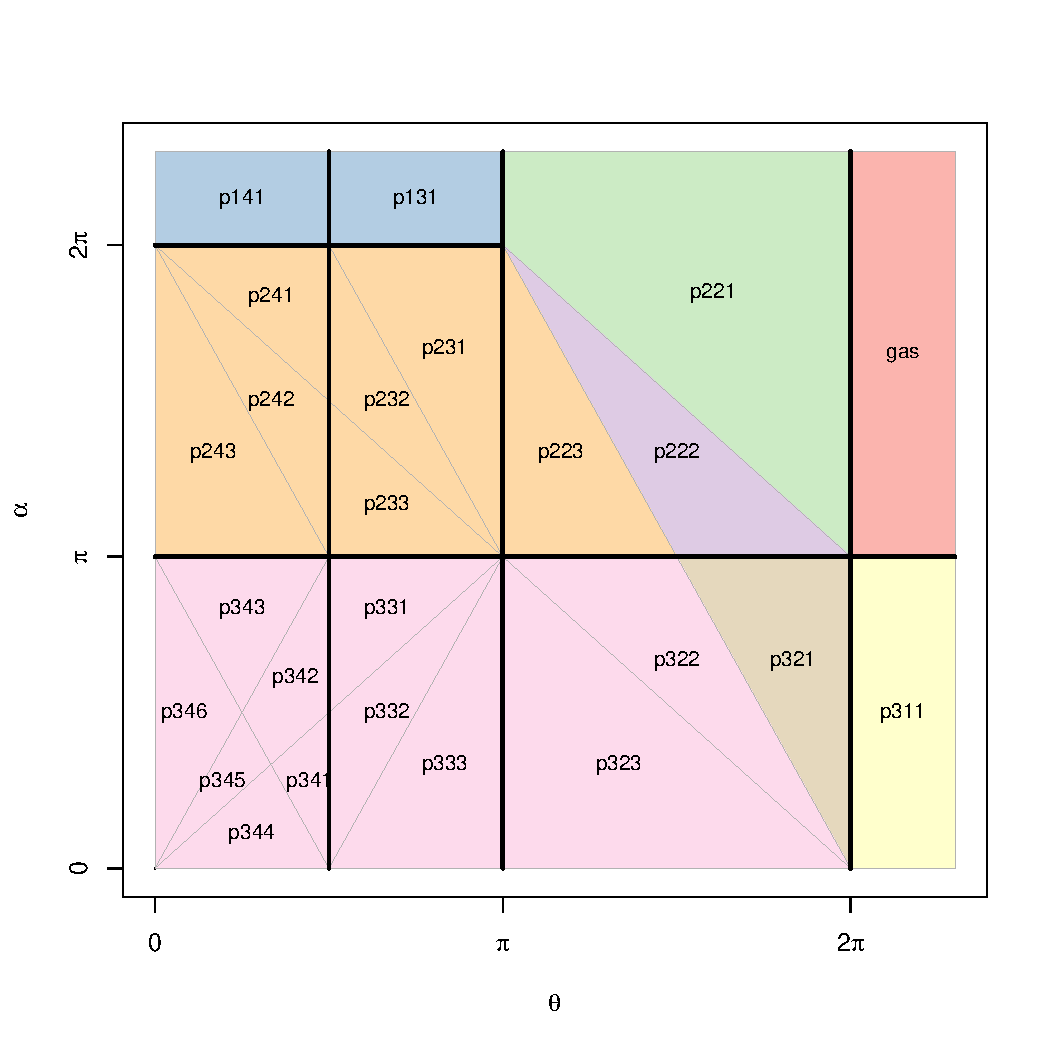
\includegraphics[width=1\textwidth]{imgs/equalRegions.pdf}
\caption{The two major parameters, call width $\alpha$ and sensor width $\theta$. Grey lines divide parameter space into a set of models which must be derived separately. Despite independent derivation the results of many models are equal. Those that are equal are filled with the same colour. Models with similar derivation are grouped together in cells which are shown with black lines. The rows and columns of these cells are used to number the models, e.g. the three models in the second row and  third column (from the top right) are called p231--p233.}
\label{f:regions}
\end{figure}



Figure~\ref{f:regions} shows the different regions with the upper right being the gas model as derived above and p141 is the model from \cite{rowcliffe2008estimating}. Parameter space is broadly split into three rows ($ \alpha \le \pi,\; \pi \le \alpha < 2\pi$ and $ \alpha = 2\pi$) and four columns ($ \theta \le \pi/2,\;  \pi/2 \le \theta \le  \pi,\;  \pi \le \theta < 2\pi$ and $\theta = 2\pi$) which define rectangular regions we will call cells. The equation for $p$ in each region is denoted by three numbers referring to rows, columns and region within that cell. 

For regions with profiles that are more complex than a circle we need to explicitly write functions for the width of the profile for every approach angle. We then use these functions to find the average profile for all approach angles by integrating across all $2\pi$ angles of approach and dividing by $2\pi$. In practice, as the models are all left/right symmetrical we can integrate across $\pi$ angles of approach and divide by $\pi$.

\subsubsection{Example derivation}

To work through one example that contains both $\theta$ and $\alpha$ we will examine p321. All other derivations are described in S1 with computer algebra scripts in S2. 

We use $x_i$ to denote the focal angle which is the angle we integrate over. The subscript $i$ distinguishes different angles. For model p321 we examine $x_1$ with  $x_1 = \pi/2$ being an approach angle directly towards the sensor (see Figure~\ref{f:xis}). \cite{rowcliffe2008estimating} use the notation $\gamma_i$ with different numbering.

\begin{figure}[t]
        \centering
        \begin{subfigure}[t]{0.34\textwidth}
                \centering
                \begin{tikzpicture}[scale=0.39]
                \fullAngleOne{0}{300}{120};
                \end{tikzpicture}
                \caption{$x_1$}
                \label{f:tikz1}
        \end{subfigure}
        
	\begin{subfigure}[t]{0.22\textwidth}
                \centering
                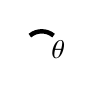
\begin{tikzpicture}[scale=0.39]
                \fullAngleTwo{0}{80}{90};
		\draw [black, ultra thick] (90 - 80/2: \angRad) arc (90 - 80/2:90 + 80/2:\angRad);
		\node [right] at (0,0) {$\theta$};
                \end{tikzpicture}
                \caption{$x_2=\pi/2$}
                \label{f:x2start}
        \end{subfigure}%%
	~ 
        \begin{subfigure}[t]{0.22\textwidth}
                \centering
                \begin{tikzpicture}[scale=0.39]
                \fullAngleTwo{0}{80}{75};
                \end{tikzpicture}
                \caption{$x_2$}
                \label{f:x2}
        \end{subfigure}
        ~ 
	\begin{subfigure}[t]{0.22\textwidth}
                \centering
                \begin{tikzpicture}[scale=0.39]
                \fullAngleTwo{0}{80}{50};
                \end{tikzpicture}
                \caption{$x_2 \rightarrow x_3$}
                \label{f:x3}
        \end{subfigure}%%
	

	\begin{subfigure}[t]{0.22\textwidth}
                \centering
                \begin{tikzpicture}[scale=0.39]
                \fullAngleThree{0}{50}{70};
                \end{tikzpicture}
                \caption{$x_3$}
                \label{f:x3}
        \end{subfigure}%%
	~
	\begin{subfigure}[t]{0.22\textwidth}
                \centering
                \begin{tikzpicture}[scale=0.39]
                \fullAngleThree{0}{50}{90};
                \end{tikzpicture}
                \caption{$x_3 \rightarrow x_4$}
                \label{f:x4}
        \end{subfigure}%%
	~ 
	\begin{subfigure}[t]{0.22\textwidth}
                \centering
                \begin{tikzpicture}[scale=0.39]
                \fullAngleFour{0}{80}{70};
                \end{tikzpicture}
                \caption{$x_4$}
                \label{f:x4}
        \end{subfigure}%%
\caption{The location of the focal angles $x_{i\in[1,4]}$ and the transitions between them. These are the angles that are integrated over to find the average profile size. In these figures, the segment shaped detection region is shown in black. The widest part of this region (the profile) is shown with a thick red line and a blue rectangle. The direction of animal movement is always downwards, as indicated by the grey arrow.}
\label{f:xis}
\end{figure}

We can see that, rotating anticlockwise, from $x_1  = \pi/2$ the detection region is $2r$ wide. However, an animal will only be detected if it approaches the detector so that as it enters the detection region the angle between the direction of approach and the direction towards the sensor is less than $\alpha/2$. The width of the profile within which the animal will be detected is therefore $2r\sin(\alpha/2)$. At $x_1  = \theta/2 + \pi/2 - \alpha/2$ we reach a point where the right hand side of the profile (relative to the approach direction) is not limited by the call angle but is limited by the detection angle instead. From here the profile width is therefore $r\sin( \alpha/2) + r\cos( x_1  - \theta/2)$. Finally, at $x_1  = 5\pi/2 - \theta/2  - \alpha/2$ an animal can again be detected from the right side of the detector; the approach angle is far enough round to see past the `blind spot' of the sensor. In this region, until $x_1  = 3\pi/2$, the width of the profile is again $2r\sin( \alpha/2)$. We have therefore characterised the profile width for $\pi$ radians of rotation (from directly towards the sensor to directly behind the sensor.) To find the average profile width for any angle of approach, we integrate these functions over their appropriate intervals of $x_1 $ and divide by $\pi$ giving us:

\begin{align}
    p321 =&\frac{1}{\pi} \left(\int\limits_{\frac{\pi}{2}}^{\frac{\pi}{2} + \frac{\theta}{2} - \frac{\alpha}{2}}2 r \sin{\left (\frac{\alpha}{2} \right )}\;\mathrm{d}x_1+\int\limits_{\frac{\pi}{2} + \frac{\theta}{2} - \frac{\alpha}{2}}^{\frac{5 \pi}{2} - \frac{\theta}{2} - \frac{\alpha}{2}}r \sin{\left (\frac{\alpha}{2} \right )} + r \cos{\left (x_1 - \frac{\theta}{2} \right )}\;\mathrm{d}x_1+\int\limits_{\frac{5 \pi}{2} - \frac{\theta}{2} - \frac{\alpha}{2}}^{\frac{3 \pi}{2}}2 r \sin{\left (\frac{\alpha}{2} \right )}\;\mathrm{d}x_1\right)\\
    p321 =& \frac{r}{\pi} \left(\theta \sin{\left (\frac{\alpha}{2} \right )} - \cos{\left (\frac{\alpha}{2} \right )} + \cos{\left (\frac{\alpha}{2} + \theta \right )}\right) \label{e:p321}
\end{align}

Then, as with the gas model, this term is used to calculate density
\begin{equation}
\label{e:gas}
D = z/vtp321
\end{equation}
We can also see what causes this model to be discontinuously different to p322. Examine the profile at $x_1 = 	\theta/2 + \pi/2$ (the profile is perpendicular to the edge of the blind spot.) We see that there is potentially a case where the left side of the profile is $r\sin( \alpha/2)$ while the right side is zero. This profile does not exist if we return to the full $2r\sin( \alpha/2)$ profile before $x_1  = \theta/2 + \pi/2$. Therefore we solve $5\pi/2 - \theta/2 - \alpha/2 <  \theta/2 + \pi/2$. We find that this new profile only exists if $ \alpha < 4\pi - 2 \theta$. This inequality defines the line separating p321 and p322.

While specifying the models had to be done by hand, the calculation of the solutions was done using SymPy \citep{sympy} in Python. The models are checked for errors with a number of tests. The models are checked against each other by checking that models which are adjacent in parameter space are equal at the boundary between them (e.g. eqn~\ref{e:p321} is equal to 2r as in the gas model when $\alpha=\pi$ and $\theta=2\pi$). Models that border $ \alpha = 0$ should have $p = 0$ when $ \alpha = 0$ and this is checked for (e.g. eqn~\ref{e:p321} is zero when $\alpha=0$ and $\theta=2\pi$). We checked that all solutions are between 0 and $2r$ and that each integral, divided by the range of angles that it is integrated over is between 0 and $2r$. These tests, as well as analytical derivations, are in supplementary script S2. The models are implemented in an R script in S3. 

\subsection{Simulation Model}

We wrote spatially explicit simulations of animal movement to validate the analytical models. By simulating animal movement and modelling a sensor surveying the population we got count data on how many animals the sensors detected. We applied the analytical models to this data and compared it to the known input animal density. We then tested whether the estimates are accurate (unbiased) and examined how precise they are.

To reduce computation effort, a single set of 100 simulations were run at the highest animal density and longest survey duration. Six sensors, with different sensor angles, were simulated during each simulation. From this one set of simulations, data for all parameter values could be computed by subsampling. To get data for lower densities, only detections of a subset of the animal population was counted. The details of each individual capture event, including the angle between the animals heading and the sensor were saved from the simulation.  From this the number of capture events can be calculated for different call widths. And finally, to achieve different survey periods, only part of the simulation was used e.g. to achieve a survey period half that of the longest survey, only the first half of the simulation was used. Therefore we get 100 replicates of each set of parameters.

Each of the 100 simulations consisted of a  \SI{7.5}{\kilo\meter} by \SI{7.5}{\kilo\meter} square (with periodic boundaries) and was populated with a density of \SI{70}{\animals\per\kilo\meter\squared} to match an expected maximum density of mammals in the wild \citep{damuth1981population}, creating a total of 3937 animals per simulation randomly placed at the start of the simulation. Animal movement was simulated with a simple movement model, characterised by a random movement distance for each discrete time step. The animals do not change direction during the simulation. The simulation lasts for $N$ steps of duration $T$ during which the animals move with an average speed, $v$. The distance travelled in each time step, $d$, was sample from a Normal distribution with mean distance, $\mu_d = vT$,  and standard deviation of $\sigma_d = vT/10$. An average speed, $v = $ \SI{40}{\kilo\meter \per \day}, was chosen as this represents the largest day range of terrestrial animals \citep{carbone2005far}, and represents the upper limit of realistic speeds. The detection radius $r$ is set to a value of 100m and simulations are run for \SI{150}{\day}.


%The directional change at the end each step can be randomly picked from a uniform distribution with a given maximum amplitude, with the basic simulation having no directional change between steps. 
%Additional simulations were also run for more complex movement models, such as, correlated random walks, and a model where a proportion of time is spent stationary. Further simulations were also run to identify the sensitivity of the sensor to changes in the radius.


The total number of capture events were counted for each simulation and each set of parameters and the analytical model applied to the results in order to estimate the density in the simulation. From this the difference between the true and estimated densities were used to evaluate the bias in the analytical models. If the analytical models are correct the mean difference between the two values were expected to converge to zero as sample size increases. For each of the 100 simulations we calculate the error (the difference between the known and estimated density) and so we got a distribution of errors which was approximately normal. We constructed 95\% confidence intervals for these normal distributions and used these to graphically test for significant differences between the true and estimated densities. The standard deviation of these distributions is our metric of precision.

To be able to produce guidelines for best practise we identified when the standard deviation of the error fell below a benchmark value which we considered acceptably precise. We chose this benchmark to be a standard deviation of less than five. In real terms this can be equated to saying that at this point if you were to sample the same area multiple times, approximately 95\% of the density estimates would be within $\pm10\%$ of the true density. From the gas model it is possible to see that the number of captures is directly proportional to the length of the survey and the speed of the animal population (eqn~\ref{e:gas}). The standard deviation of estimate error, and therefore the  appropriate survey duration for use in the field is closely linked to the number of captures. Rather than looking at the animal speed and survey time separately we studied them together as the average distance moved by the animal within the duration of the survey. 


% I edited this, but need to check it's correct. The survey length is subsampled rather than the average distance travelled?


Four models, p141 (REM model), p343, p221, and p322, were selected to demonstrate how the precision and accuracy varied with model inputs. These models were chosen as they represent one model from each quadrant of Figure~\ref{f:regions}. The accuracy and precision of all models should be similar to these.


\section{Results}

\subsection{Analytical model}

Model results have been derived for each region in Figure~\ref{f:regions} with all models except the gas model and p141 being newly derived here. However, many models, although derived separately, have the same expression for $p$. Figure~\ref{f:equalModelResults} shows the expression for $p$ in each case. The general equation for density, using the correct model for $p$ is then
\begin{equation}
\label{e:D}
	D = z/pvt.
\end{equation}

Although more thorough checks are performed in S3, it can be seen that all adjacent expressions in Figure~\ref{f:equalModelResults} are equal when expressions for the boundaries between them are substituted in.


\begin{figure}
\centering
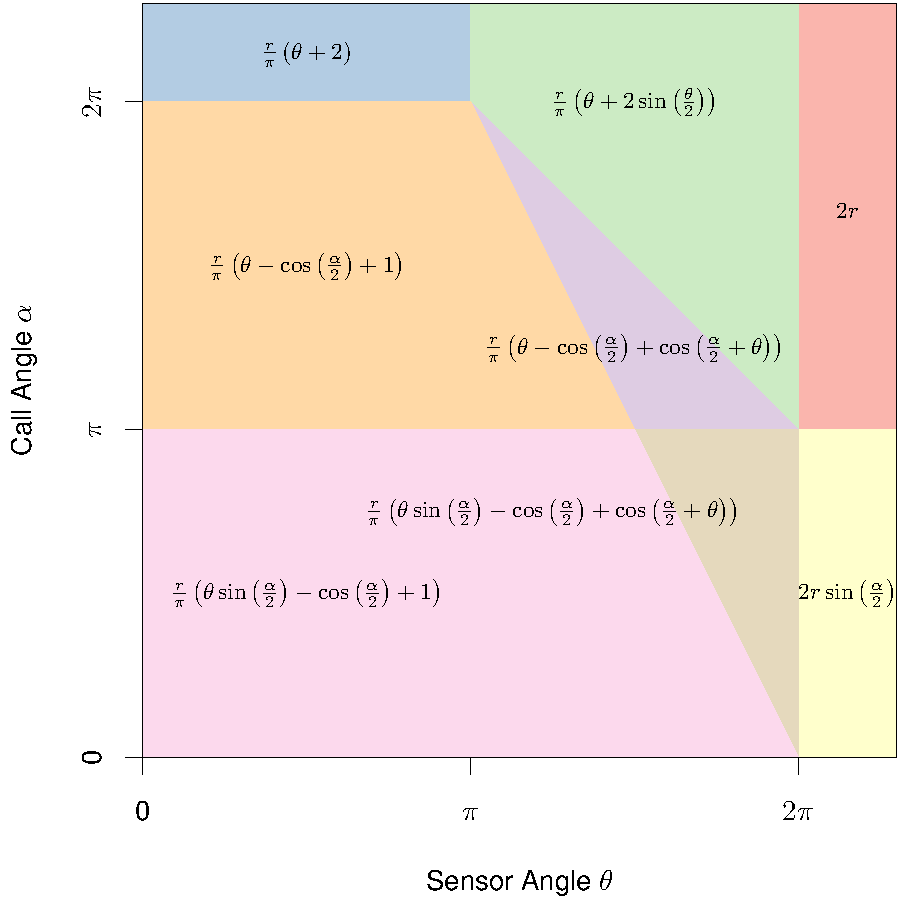
\includegraphics[width=1\textwidth]{imgs/equalModelResults.pdf}
\caption{The derived expressions of for calculating the average profile width $p$. Despite independent derivation, many models result in the same expression. These are collected together and presented as one block of colour.}
\label{f:equalModelResults}
\end{figure}



\subsection{Simulation model}

None of the estimated densities from the simulation showed significant deviation from the true density in the simulation (Figure~\ref{f:ModelBias}). The precision of the models do vary however. The standard deviation of the error is strongly related to the call and sensor width (Figure~\ref{f:StandardDevaition}), such that larger widths have greater precision. Even the models with small call and sensor widths have an acceptable level of precision relative to our benchmark when the full length simulation is used. 

\begin{figure}
	\centering
	%\begin{subfigure}[t]{0.5\textwidth}
	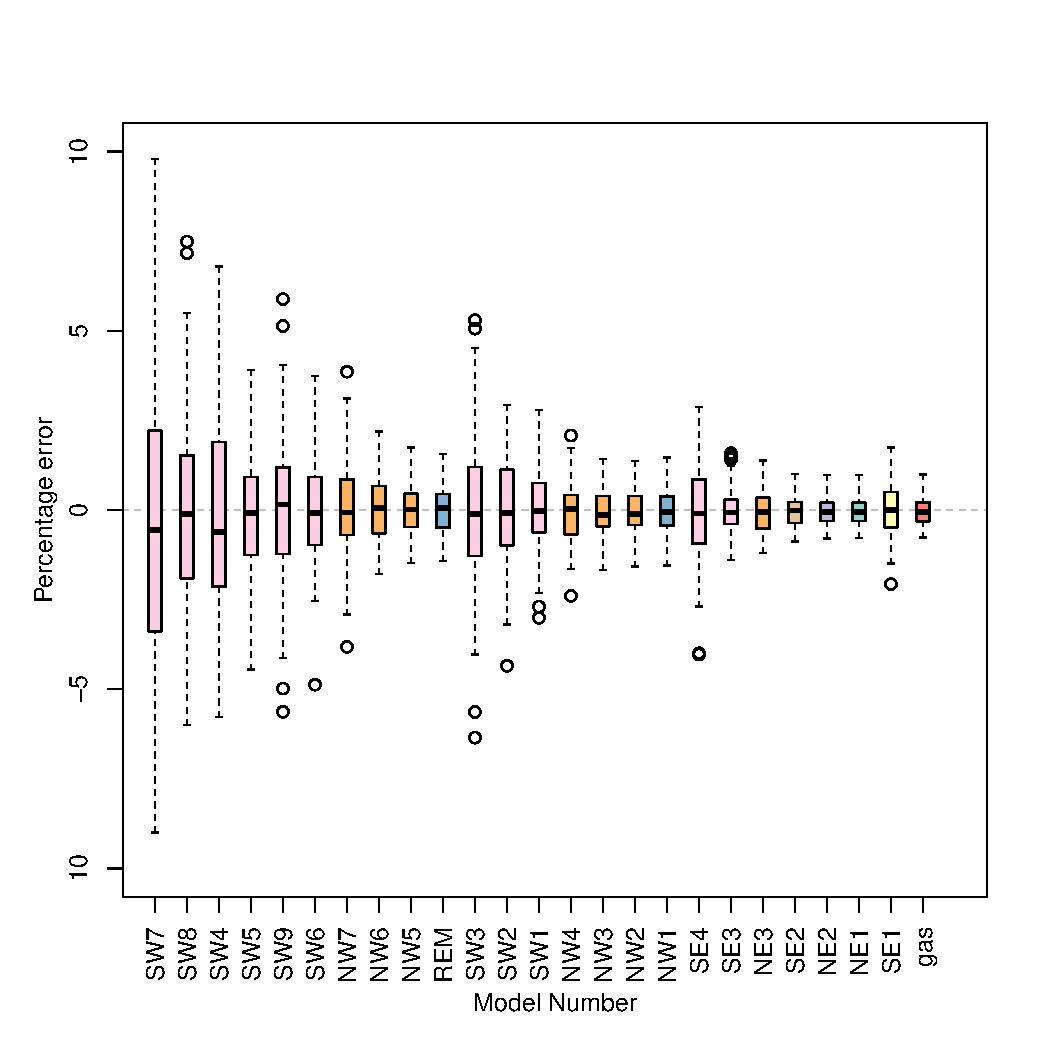
\includegraphics[width=1\textwidth]{imgs/AverageModelBias.pdf}
	\caption{Bias}
	\label{f:ModelBias}
%	\end{subfigure}
%	~

	\caption{Percentage error and standard deviation of analytical model calculated from the simulation when settings are: $r = $\SI{100}{\meter}; $T = $\SI{150}{\day}; $v = $ \SI{40}{\kilo\meter\per\day}; $D=$\SI{70}{\animals\per\kilo\meter\squared}; and with angles varying between models. The average percentage error generated by the simulation per model derivation, shown with 95\% confidence intervals.}
	\begin{comment} 
	p344: $\alpha$= 0.3491; $\theta$=0.2856.  
	 p345: $\alpha$= 0.3491; $\theta$=0.5712.
	 p346: $\alpha$= 0.3491; $\theta$=0.8568.
	 p244: $\alpha$= 0.3491; $\theta$=1.4280.
	 p242: $\alpha$= 0.3491; $\theta$=1.7136.
	 p241: $\alpha$= 0.3491; $\theta$=2.5704.
	 p141: $\alpha$= 0.3491; $\theta$=3.1416.
	 p341: $\alpha$= 0.6981; $\theta$=0.2856. 
	 p342: $\alpha$= 0.6981; $\theta$=0.8568.
	 p333: $\alpha$= 1.0472; $\theta$=0.2856.      
	 p332: $\alpha$= 1.0472; $\theta$=0.8568.
	 p331: $\alpha$= 1.0472; $\theta$=1.4280.
	 p233: $\alpha$= 1.0472; $\theta$=1.7136.
	 p232: $\alpha$= 1.0472; $\theta$=2.5704.
	 p231: $\alpha$= 1.0472; $\theta$=2.8560.
 	p131: $\alpha$= 1.0472; $\theta$=3.1416.
 	p323: $\alpha$= 1.7453; $\theta$=0.2856.  
 	p322: $\alpha$= 1.7453; $\theta$=1.4280.
 	p223: $\alpha$= 1.7453; $\theta$=1.7136.       
 	p321: $\alpha$= 2.7925; $\theta$=1.4280.         
 	p222: $\alpha$= 2.7925; $\theta$=1.7136. 
 	p221: $\alpha$= 2.7925; $\theta$=2.8560.       
 	p311: $\alpha$= 3.1416; $\theta$=0.2856.  
 	Gas: $\alpha$= 3.1416; $\theta$=2.8560.                                      
	\end{comment}
\end{figure}


Neither the average distance travelled by an animal during the survey, or animal density, had a significant impact on the accuracy of the model (Figure~\ref{f:distanceDensity}). However, both these factors affected the precision of estimates. The precision of estimates increased with distance travelled, Figure~\ref{f:Distance}. The precision of the model fell below the benchmark when the animals on average moved less than \SI{40}{\kilo\meter}, \SI{55}{\kilo\meter}, \SI{25}{\kilo\meter} and \SI{25}{\kilo\meter} for models p141, p343, p221, and p322 respectively. The density of the population also affected the precision of the estimates with larger population densities being associated with greater precision (Figure~\ref{f:Density}). 
%The density of the populations becomes a limiting factor for the precision of the model if it falls below %VALUE NOT CALCULATED YET% . 

\begin{figure}[t]
        \centering
	\begin{subfigure}[t]{0.5\textwidth}
		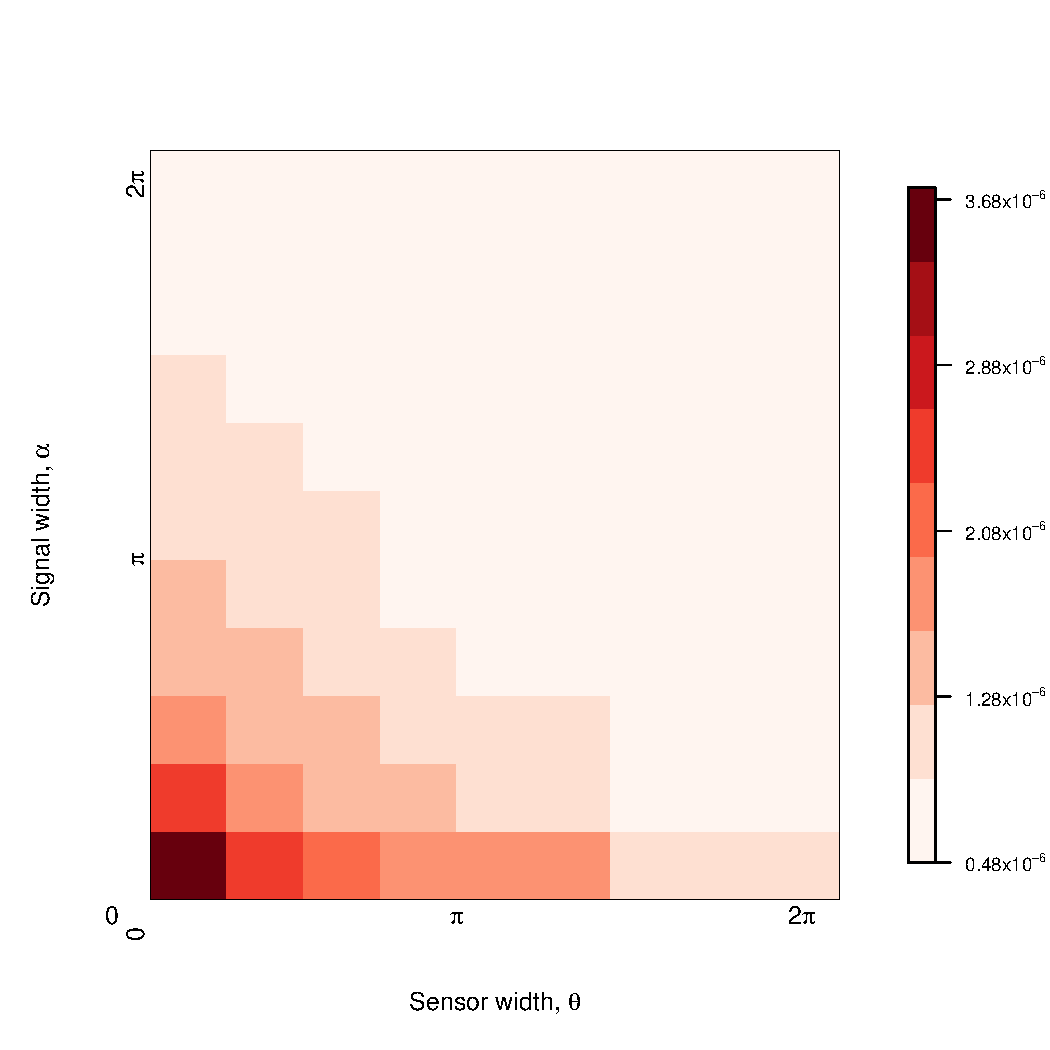
\includegraphics[width=1\textwidth]{imgs/ResultStandardDeviation.pdf}
		\caption{Angle of detector}
		\label{f:StandardDevaition}
	\end{subfigure}
	~
	 \begin{subfigure}[t]{0.5\textwidth}
                \centering
		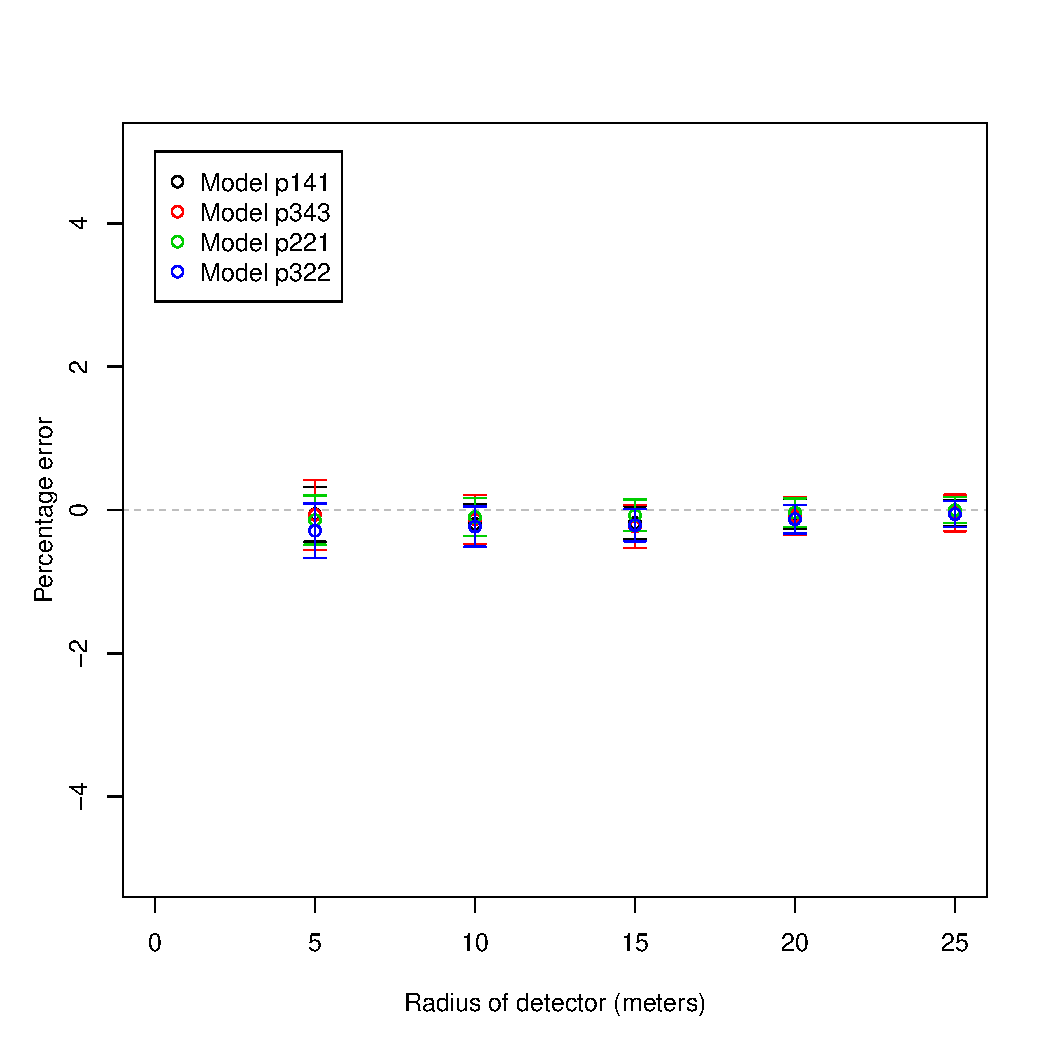
\includegraphics[width=1\textwidth]{imgs/ResultsRadii.pdf}
                \caption{Radius of the detector}
                \label{f:Radii}
        \end{subfigure}
        
        \caption{ The standard deviation of the percentage error for sensor, and call angles between 0 and $2\pi$ (A), and
        the percentage error of the estimate with increasing radius of the detector with 95\% confidence intervals (B).
        } 
\end{figure}

\begin{figure}[t]
        \centering
        \begin{subfigure}[t]{0.5\textwidth}
                \centering
		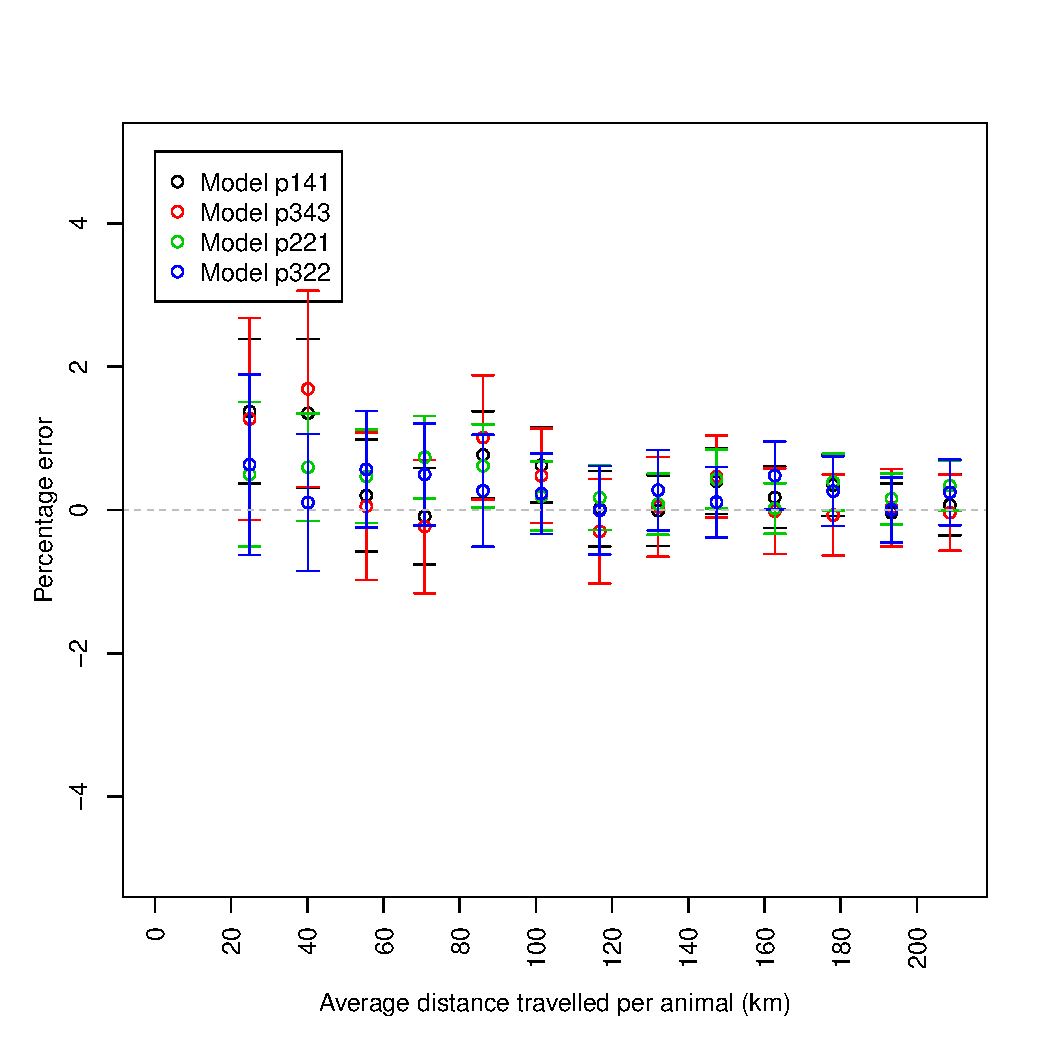
\includegraphics[width=1\textwidth]{imgs/ResultsDistanceSubsample.pdf}
                \caption{Distance}
                \label{f:Distance}
        \end{subfigure}
        ~ 
        \begin{subfigure}[t]{0.5\textwidth}
                \centering
		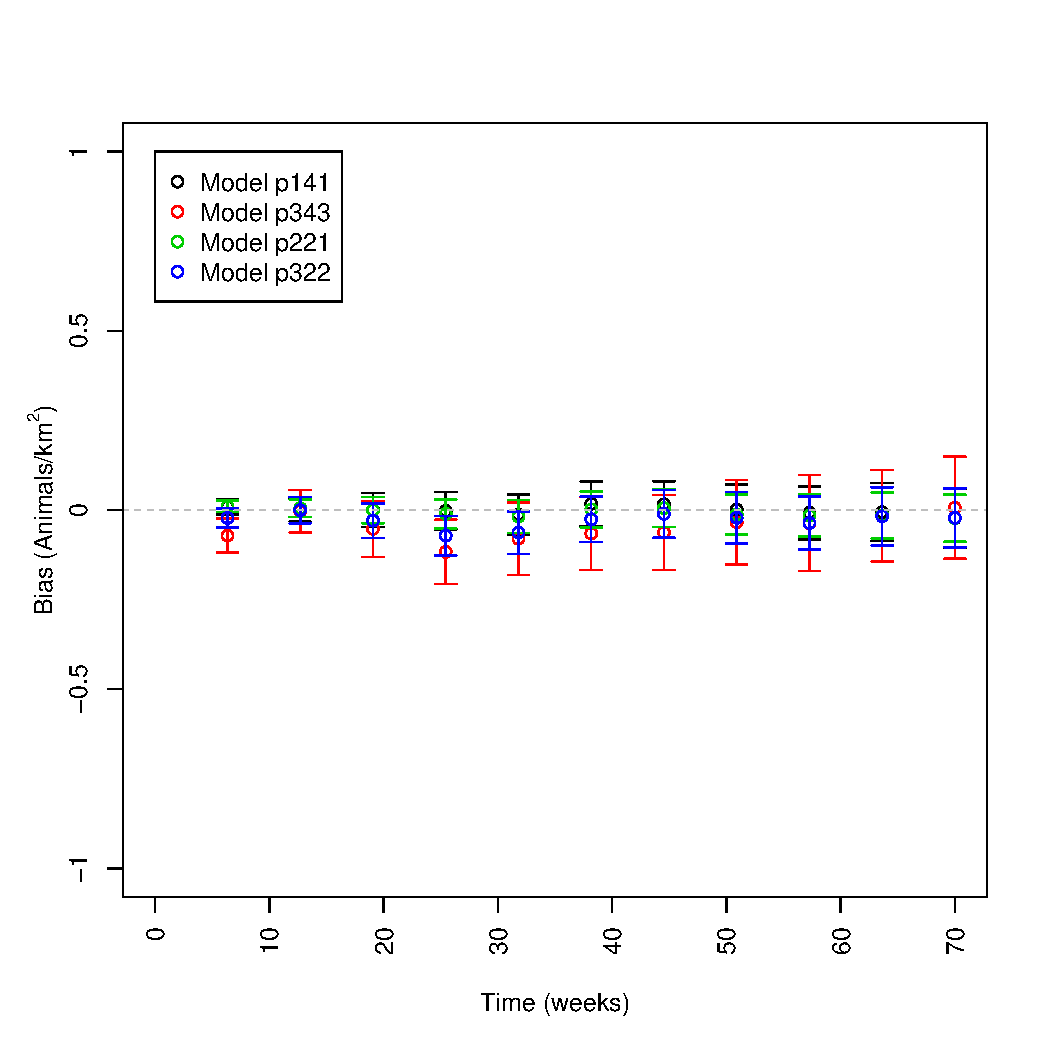
\includegraphics[width=1\textwidth]{imgs/ResultsDensitySubsample.pdf}
                \caption{Density}
                \label{f:Density}
        \end{subfigure}
	\caption{Discrepancy between known simulation density and estimated density with increasing animal movement (A) and animal density (B) with 95\% confidence intervals.}
	\label{f:distanceAnimal}
\end{figure}


If an animal displays a start-stop move of movement this will not effect the accuracy, or the precision, of the estimates as long as the average speed over the length of the study is known (Figure~\ref{f:Perch}). 

The range of the camera has an affect of the precision of the estimator, but not on the accuracy. The precision remains relatively small even with a range as small as 5 meters (Figure~\ref{f:Radii}). 


\begin{figure}[t]
        \centering
        \begin{subfigure}[t]{0.5\textwidth}
                \centering
		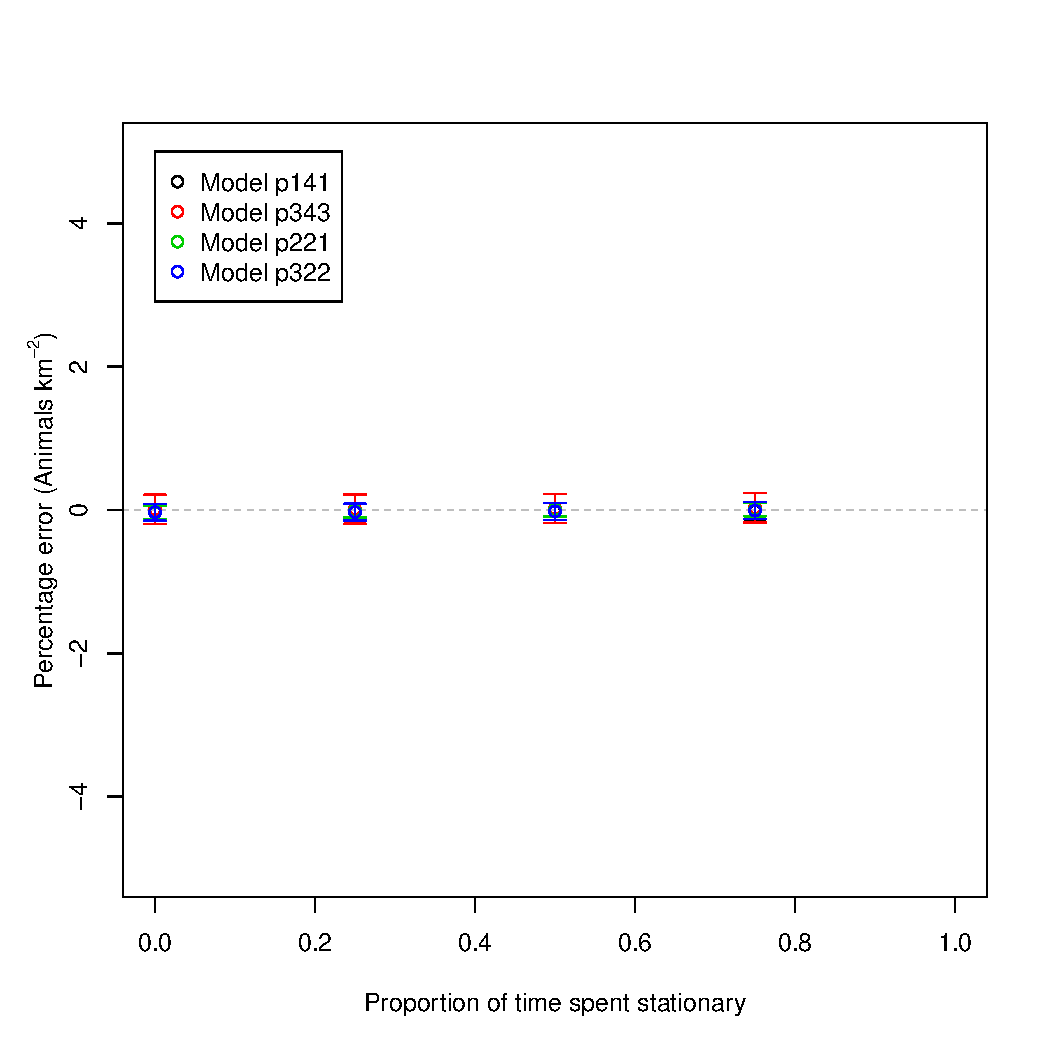
\includegraphics[width=1\textwidth]{imgs/ResultsPerching.pdf}
                \caption{Proportion of time spent stationary}
                \label{f:Perch}
        \end{subfigure}
        ~ 
	\begin{subfigure}[t]{0.5\textwidth}
                \centering
		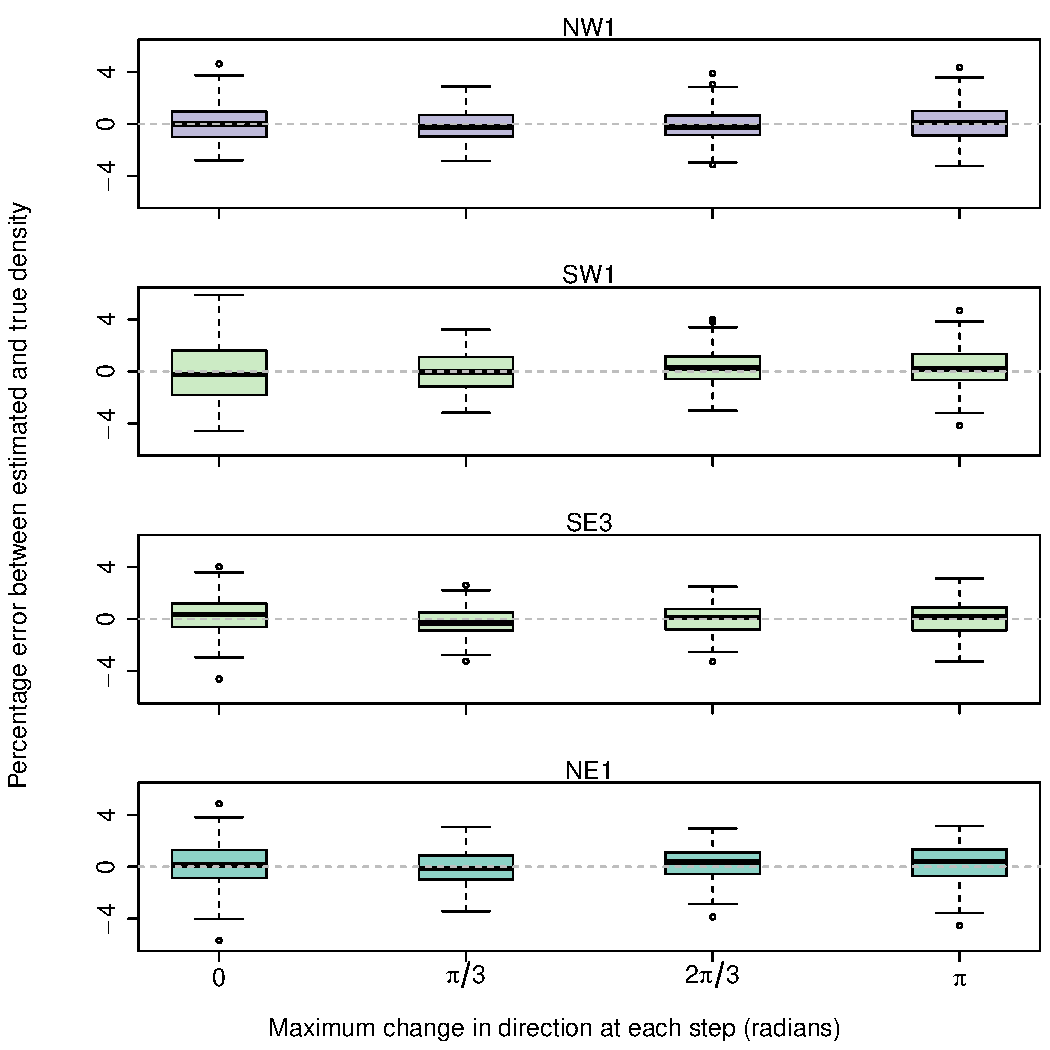
\includegraphics[width=1\textwidth]{imgs/ResultsTort.pdf}
                \caption{Angle of correlated walk}
                \label{f:Tort}
        \end{subfigure}
	\caption{Discrepancy between known simulation density and estimated density when animals spend increasing proportion of time stationary (A) and when they move with different types of correlated walk (B) with 95\% confidence intervals.}
	\label{f:distanceMovement}
\end{figure}

\begin{comment}
\begin{itemize}
%\item Bias is approximately zero for all models as demonstrated by simulation: 
%	\begin{itemize}
%	\item At a given speed, density, sampling effort, sensor radius, and a given movement strategy
%	\end{itemize}	


\item The expected number of captures will vary, dependent on the system that is being monitored and how it is monitored. This will affect the precision of the estimated: 
	\begin{itemize}
	\item Animal movement strategy
	\item Speed of movement
	\item Density of the animal
	\item Sampling effort
	\item Radius of the sensor
	\end{itemize}
\end{itemize}
\end{comment}



\section{Discussion}

%• Discussion: Point out the importance of the results and place them in the context of previous studies and in relation to the application of the work (expanding on the Synthesis and applications section of the Summary). Where appropriate, set out recommendations for management or policy.

We have developed a number of models that can be used to estimate density from acoustic and optical sensors. This has entailed a generalisation of the gas model and the model in \cite{rowcliffe2008estimating} to be applicable to any combination of sensor width and call directionality. We have used simulations to show, as a proof of principle, that these models are accurate and precise. %We have broken  the ideal gas assumptions of animal movement and still retained accurate results, although precision is lowered. Finally we have given some general advise on best practice, although this is given based on similar assumptions those used in the derivation in the models.

These model are therefore available for the estimation of density of a number of taxa of importance to conservation, zoonotic diseases and ecosystem services. The models are suitable for certain groups for which there are currently no, or few, effective methods for density estimation. 

Importantly the methods are noninvasive and do not require human marking (as required for mark-recapture models). This makes them suitable for large, continuous monitoring projects with limited human resources. It also makes them suitable for sensitive species or species that are difficult or dangerous to catch.

Although we have used simulations to validate these models, much more robust testing is needed. Although difficult, proper field test validation would be required before the models could be fully trusted. Note, however, that the gas model and model of \cite{rowcliffe2008estimating} have been been field tested and many of the assumptions between these models and those derived here are the same. As the utility of the models is that they can be used with taxa that are difficult to study with other methods, there are not many obvious groups that have reliable, gold standard estimates of density from other methods that could then be used to validate these models.

As easier way to continue to evaluate the models is to run more extensive simulations which break the assumptions of the analytical models. The main element that cannot be analytically treated is the complex movement of real animals. Therefore testing these methods against true animal traces, or more complex movement models would be useful.

There are many possible extensions to these models. As has been noted before \citep{rowcliffe2008estimating,Hutchinson_Waser_2007} altering the equations to estimate animal density of group living species is relatively simple. However, the models herein would have to be carefully rederived to account for group living as directional calls are not considered in previous work, and may have important effects.

The original gas model was formulated for the case where both the animal population and the sensors are moving. Indeed any of the models with animals that are equally detectable in all directions ($\alpha = 2\pi$) can be trivially expanded for moving by substituting the sum of the average animal velocity and the sensor velocity for $v$ as used here. However, when the animal has a directional call, the extension becomes much less simple. The approach would be to calculate again the mean profile width. However, for each angle of approach, one would have to average the profile width for an animal facing in any direction (i.e. not necessarily moving towards the sensor) weighted by the relative velocity of that direction.

An interesting, and so far unstudied problem, is edge effects caused by trigger delays (the delay between sensing an animal and attempting to record the encounter) and time expansion acoustic detectors which repeatedly turn on an off during sampling. Both of these have potential biases as animals can move through the detection region without being detected. The models herein are formulated assuming constant surveillance and so the error quickly becomes negligible.




\begin{comment}

\begin{itemize}
\item Developed a number of models that can be used to estimate density from acoustic and optical sensors 
\item These models are accurate 
\item Implications for best practice:
	\begin{itemize}
	\item Densities of above X converge quickly to a stable mean
	\item Animals which have an average speed of greater then X 
	\item Surveys of at Xhrs of effort produce stable results
	\end{itemize}
\item Aspirational stuff for the future:
	\begin{itemize}
	\item Consider animals moving in groups
	\item Incorporating more realistic movement strategies
	\item Moving detectors
	\item Trigger delays and time expansion
	\end{itemize}
\end{itemize}

\end{comment}


%\section{Acknowledgements}



%\section{Data Accessibility}




\bibliographystyle{mee.bst}	
\bibliography{lucas-moorcroft-etal-refs.bib}	


\end{document}
		
